\documentclass[aspectratio=1610]{beamer}
\usepackage[utf8]{inputenc}
\usepackage{multicol}
\usepackage[czech]{babel}
\usepackage{amsmath}
\usepackage{csquotes}

\usepackage[sfdefault]{roboto}
\usepackage[T1]{fontenc}

\title{Test č. 1}
\date{WBA | 5. hodina}
\author[Cajthaml]{Matěj Cajthaml}

\usetheme{material}

\usePrimaryCustom

\begin{document}

\begin{frame}
\titlepage
\end{frame}




\begin{frameImg}[width]{img/pray.jpg}
    \vspace*{60mm}
    \begin{cardTiny}
        \vspace*{\fill}
        \begin{center}
            \textbf{Písemné zkoušení}
        \end{center}
    \end{cardTiny}
\end{frameImg}


\begin{frame}{Informace k testu}
    \begin{cardTiny}
        \begin{flushleft}
            Bodový základ: 17 bodů (+3 body)

            Počet otázek: 11 (+2)

            Na "čtyřku"~~stačí 7 bodů.

            Neexistují půlbody. Nepodvádějte, nefoťte, nemluvte.

            \vspace{2ex}

            Nepsat červenou barvu.

            Pište čitelně.

            \vspace{2ex}

            Vyplnit příjmení a jméno. Hodnocení nechat prázdné.

            Za zadáním otázky je políčko na počet bodů - nevyplňovat.

            \vspace{2ex}
            Zapisování správné odpovědi.
        \end{flushleft}
    \end{cardTiny}
\end{frame}

\begin{frame}{Informace k otázkám}
    \begin{cardTiny}
        \begin{flushleft}
            Řiďte se nápovědou u otázky.

            Vše může být pravda i nepravda.  

            Otevřené otázky.
        \end{flushleft}
    \end{cardTiny}

    \begin{cardTiny}
        \begin{flushleft}
            Při nějakém problému se přihlašte.
        \end{flushleft}
    \end{cardTiny}
\end{frame}



\begin{frame}
    \begin{center}
        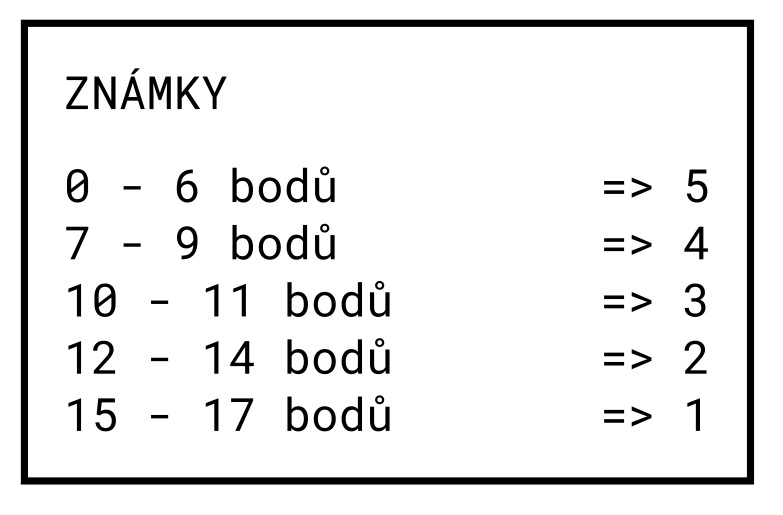
\includegraphics[width=0.8\textwidth]{img/test-1-hodnoceni.png}
    \end{center}
\end{frame}


\begin{frameImg}[width]{img/thinking.jpg}
    \vspace*{60mm}
    \begin{cardTiny}
        \vspace*{\fill}
        \begin{center}
            \textbf{Hodně štěstí!}
        \end{center}
    \end{cardTiny}
\end{frameImg}

\begin{frameImg}[width]{img/rate.png}
    \vspace*{60mm}
    \begin{cardTiny}
        \vspace*{\fill}
        \begin{center}
            \textbf{Jak Vám to šlo? / Co si o testu myslíte?}
        \end{center}
    \end{cardTiny}
\end{frameImg}


\end{document}